\subsection{NeuroGEARS}

NeuroGEARS is a UK technology company that helps research institutions adopt
state-of-the-art technologies to develop innovative biomedical research.  The
director of NeuroGEARS, Dr.~Goncalo Lopes, is the inventor, and his company is
the main supporter, of Bonsai, a reactive visual programming language that
powers thousands of experiments around the world. 
The primary goal of NeuroGEARS is to advance scientific research, share knowledge,
and empower researchers with free and accessible tools\footnote{
The NeuroGEARS business model focuses on:

\begin{description}

	\item[Open Source:] NeuroGEARS mainly focuses on developing and
distributing open-source tools for electrophysiology research. They release
these tools under open-source licenses, such as the MIT License, which allows
anyone to use, modify, and distribute the software and hardware freely.

	\item[Collaboration:] NeuroGEARS fosters a collaborative environment where
researchers and engineers contribute to the development of tools and share
their creations with the community. This collaborative effort enables the
refinement and expansion of the tools distributed by NeuroGEARS.

	\item[Community Support:] NeuroGEARS relies on the support of the
scientific and research community, which benefits from the tools they provide.
This support can come in the form of contributions, feedback, and engagement
from scientists and researchers who use their tools.

	\item[Educational Workshops and Training:] Hosting workshops, training
sessions, and educational events related to advanced experimentation generates
revenue for NeuroGEARS.

	\item[Grants and Donations:] NeuroGEARS seeks funding through grants,
donations, or sponsorship from institutions, organizations, and individuals who
support open science and open-source initiatives. These funds are typically
used to cover operational costs, further tool development, and support the
community.

\end{description}

}.

\subsection{Needs for advanced experimention}

The vast majority of experiments that people (and specially scientists) perform
use simple artificial stimuli, are open loop, short duration, only test simple
stereotypical behaviors in their subjects and they are controled by simple
pre-defined rules.

\begin{comment}
In contrast, in collaboration with the SWC and the Gatsby Unit we are
performing a new kind of experiments with naturalistic stimulation, close-loop
control, long durations and complex natural behaviors. In addition these experiments are intelligently controlled by machine learning algorithms making statistical inferences about subjects' hidden states.
\end{comment}

One reason that hinders people from performing more complex experiments is the
unavailability of hardware, easy-to-use software and expertise for advanced
experimentation. However, this is currently changing with the appearence of
disrupting open-source technologies.

In 2010, Josh Siegel and Jakob Voigt created Open Ephys to develop open-source
hardware for electrophysiological research to benefit the neuroscience research
community.  Open Ephys has since grown and expanded its contributions to the
field. This technology has been highly disruptive, by challenging the status
quo, reducing costs, promoting collaboration, and enhancing transparency,
offering significant benefits to the scientific community\footnote{

A few reasons why Open Ephys has been a highly disruptive technology:


\begin{description}

	\item[Cost-Effective Solutions:] Open Ephys provides open-source hardware and software tools that are often more cost-effective than traditional, proprietary solutions. This affordability disrupts the market by making high-quality electrophysiology tools accessible to researchers and institutions with limited budgets.

	\item[Democratizing Access:] By offering free, open-source tools, Open Ephys democratizes access to advanced electrophysiology equipment and data analysis software. This levels the playing field, allowing a broader range of researchers and institutions to conduct high-quality experiments.

	\item[Customization and Flexibility:] Open Ephys' open-source nature allows users to customize and adapt the tools to their specific research needs. This flexibility disrupts the one-size-fits-all approach of proprietary systems and empowers researchers to tailor their equipment and software to their experiments.

	\item[Community Collaboration:] Open Ephys fosters collaboration among a global community of researchers, scientists, and engineers. This collective effort results in the continuous improvement and development of electrophysiology tools, driving innovation within the field.

	\item[Transparency and Accountability:] Open-source software and hardware are transparent, meaning the code and designs are open for scrutiny. This transparency can lead to more reliable, secure, and accountable solutions, disrupting the closed, opaque nature of some proprietary systems.

	\item[Reduction of Vendor Lock-In:] Proprietary systems can create dependency on specific vendors. Open Ephys reduces this lock-in by offering alternatives and encouraging vendor independence. Researchers are not limited to a single supplier, giving them more control.

	\item[Rapid Development and Updates:] The open-source community's collaborative nature can lead to faster development and frequent updates. Researchers can benefit from new features and improvements more quickly, disrupting the slower development cycles of some proprietary systems.

	\item[Innovation and Experimentation:] The open-source approach encourages innovation and experimentation. Researchers and developers can build upon existing tools, leading to the creation of novel solutions and techniques that challenge the status quo.

	\item[Knowledge Sharing:] Open Ephys promotes the sharing of knowledge and best practices within the electrophysiology community. This open exchange of information accelerates research progress and disrupts traditional silos of knowledge.

	\item[Longevity and Sustainability:] Open-source projects tend to be community-driven and can outlast the involvement of individual creators or companies, ensuring the longevity of tools and solutions.

\end{description}

}

Another barrier to perform complex experiments is the unavailability of
easy-to-use open-source software to control them. To address this limitation,
in 2011, while doing his PhD, Goncalo Lopes started developing Bonsai. Its
adoption by the scientific and non-scientific community was extraordinarly
large (see Fig.~\ref{fig:bonsai}). Thus, in 2017, after completing his PhD,
Dr.~Lopes created NeuroGEARS Ltd, to focus on the open-source development and
dissemination of Bonsai.

\begin{figure}
	\begin{center}
		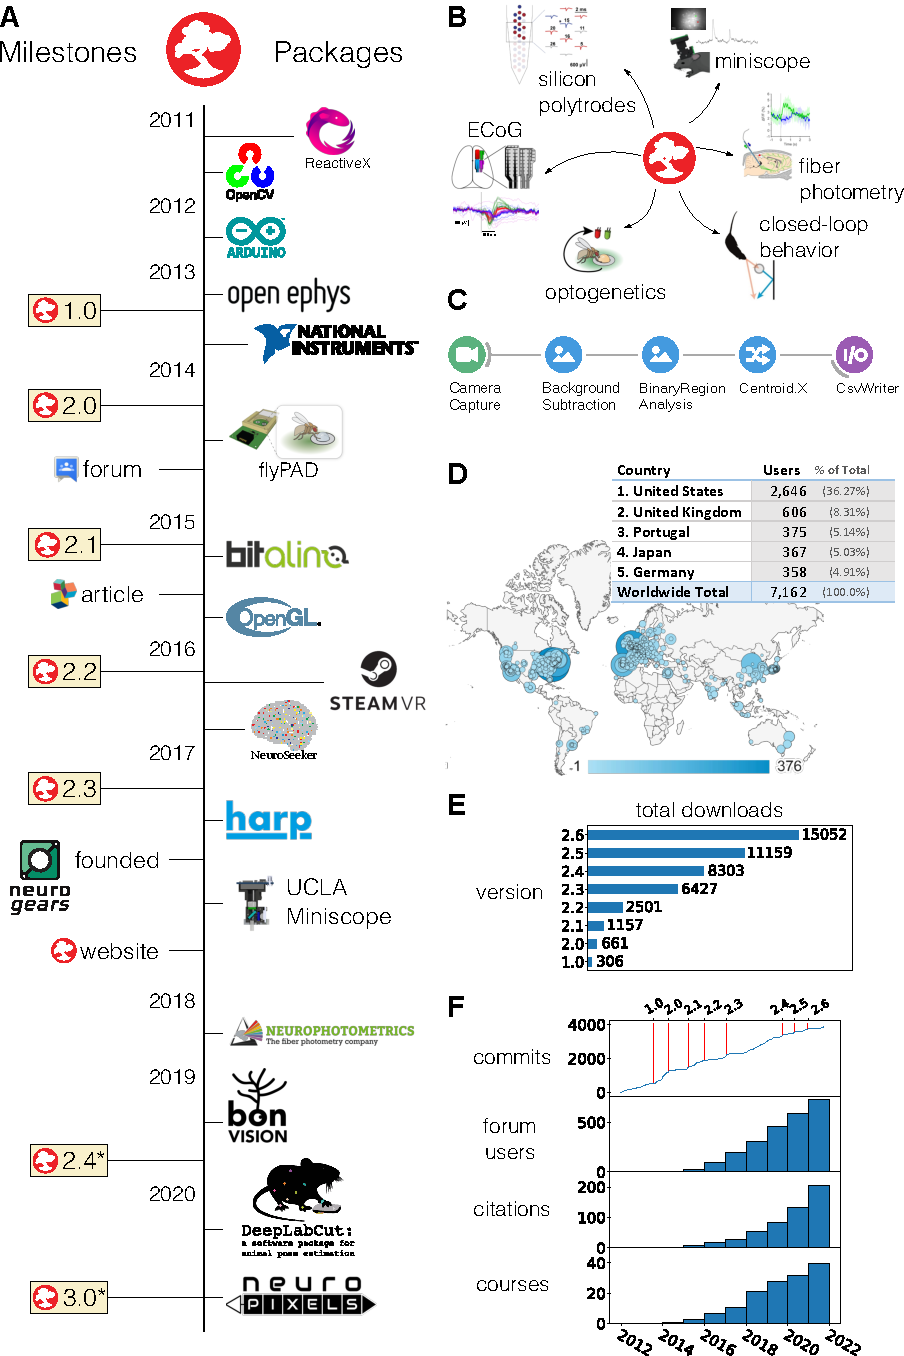
\includegraphics[width=3in]{figures/roadmap-bbsrc-3x.pdf}
	\end{center}
	\caption{Bonsai: development timeline and usage statistics.}
	\label{fig:bonsai}
\end{figure}

Yet, another missing for the implementation of advanced experiments is the
dissemination of expertise in this type of experimentation. This dissemination
is at the core of our proposal.

\subsection{NeuroGEARS-SWC-GCNU collaboration}

NeuroGEARS has been working with the Sainsbury Wellcome Centre and the Gatsby
Computational Neuroscience Unit, both at University College London, for more
than two years developing hardware and software technology for unrestrained,
long-duration, naturalistic, closed-loop and intelligent experimentation in
neuroscience by combining its engineering expertise with the machine learning
and experimental neuroscience research experience of its academic partners.
Together they are opening a new chapter on neuroscience experimentation.

\subsection{Technology dissemination}

The technology that NeuroGEARS is developing in collaboration with the SWC and
the Gatsby Unit is specialised to support neuroscience experiments in rodents.
We offer to generalise this technology to support a wider range of experimental
setups and to distribute it openly to experimentalists around the world.

The potential of disseminating this technology are enormous. Academically,
this technology is allowing to probe systems in natural regimes that cannot
be studied with traditional simpler experiments, and to study these systems in
unprecedented detail. For example in the 24/7 experiments that we
are developing at the SWC we can study foraging in naturalistic environments
where we can control environmental experimental variables (e.g., food delivery)
with great precision, while we record and manipulate neural activity.

The business applications of these technologies are also very large. For
instance in the pharmaceutical industry, these technologies could allow
unprecedented efficiency for automatic drug testing \ldots Another application
appears in the domain of personalised healthcare \ldots

In addition, long-duration, naturalistic and close-loop experiments will
incentivize several adjacent industries, like those of computer storage (to
save the very large amounts of data produced by these experiments), or the
industry of physiological measurement devices (key components in our
experiments).

Furthermore, the novel datasets that our experiments are producing are also
incentivizing academic research in, for example, machine learning algorithms to
process real time time series.

\subsection{Proposal aim}

The current joint work between NeuroGEARS, the SWC and the Gatsby Unit is to
build infrastructure to perform long-duration, naturalistic, close-loop and
intelligent experiments in order to investigate a specifics problems in the
real systems neuroscience. We aim at distributing hardware, software and
machine learning technology to allow a wider range of long-duration,
naturalistic and close-loop experiments.
